\newgeometry{left=1in, right=1in,top=1in, bottom=0in}
{

\DeclareFixedFont{\titlefont}{T1}{ppl}{b}{}{0.5in}
\DeclareFixedFont{\subtitlefont}{T1}{ppl}{m}{it}{0.4in}
\DeclareFixedFont{\authorfont}{T1}{ppl}{sb}{}{0.3in}
\DeclareFixedFont{\versionfont}{T1}{ppl}{}{}{0.2in}
\DeclareFixedFont{\downloadfont}{T1}{ppl}{}{}{0.15in}

\definecolor{mytan}{HTML}{F6D5A8}
\pagecolor{mytan}

\colorlet{greytitle1}{black!95!}
\colorlet{greytitle2}{black!65!}
\colorlet{greytitle3}{black!75!}

\thispagestyle{empty}
\begin{flushright}
  \color{greytitle1}
  \titlefont High School Informatics\\[9pt] 
  \color{greytitle2}
  \subtitlefont for complete beginners\\[24pt]
  \color{greytitle3}
  \authorfont Gavin Sinclair
  \vfill
  \versionfont \BookVersionString \\[6pt] \BookVersionDate \\[12pt]
  \color{greytitle2}
  \downloadfont \BookDownloadText
  \vfill
\end{flushright}

\begin{center}
  \begin{tikzpicture}
    \node[scope fading=north, inner sep=0pt, outer sep=0pt]{
       \makebox[\textwidth]{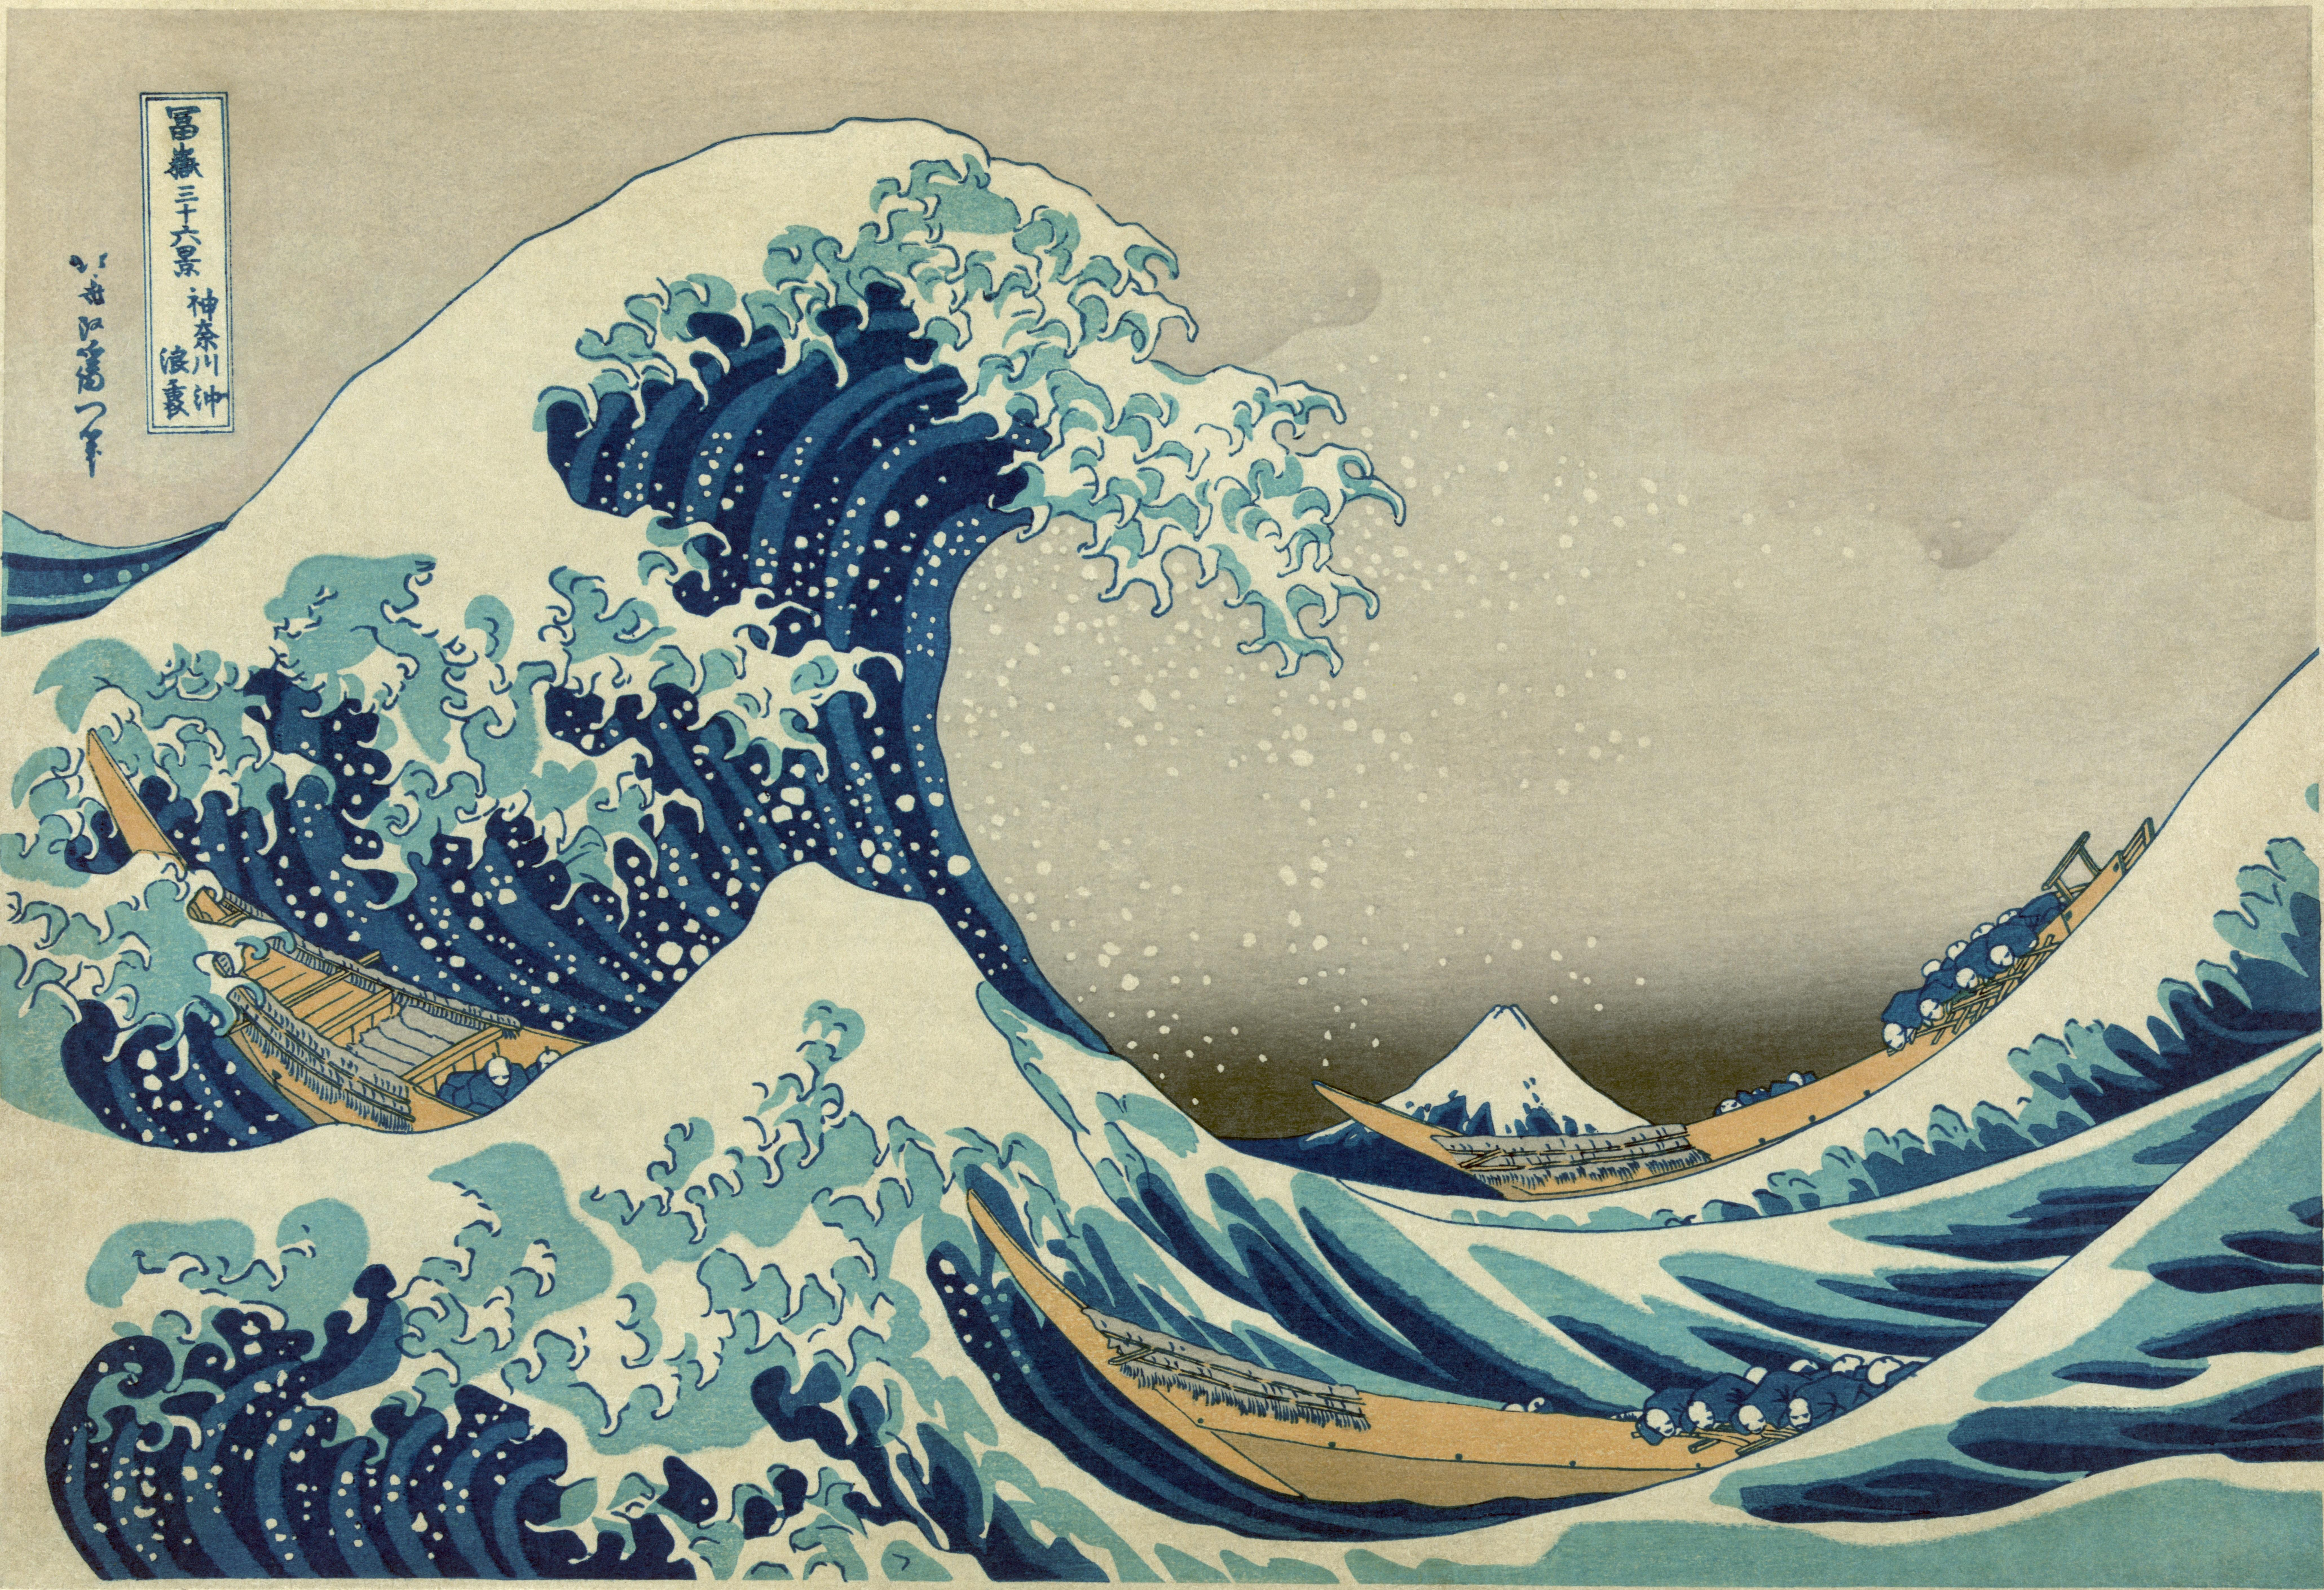
\includegraphics[width=\paperwidth]{images/kanagawa-wave.jpg}}
     };
   \end{tikzpicture}
 \end{center}

}
